\subsection{Model Validation}

\begin{figure}
  \centering
    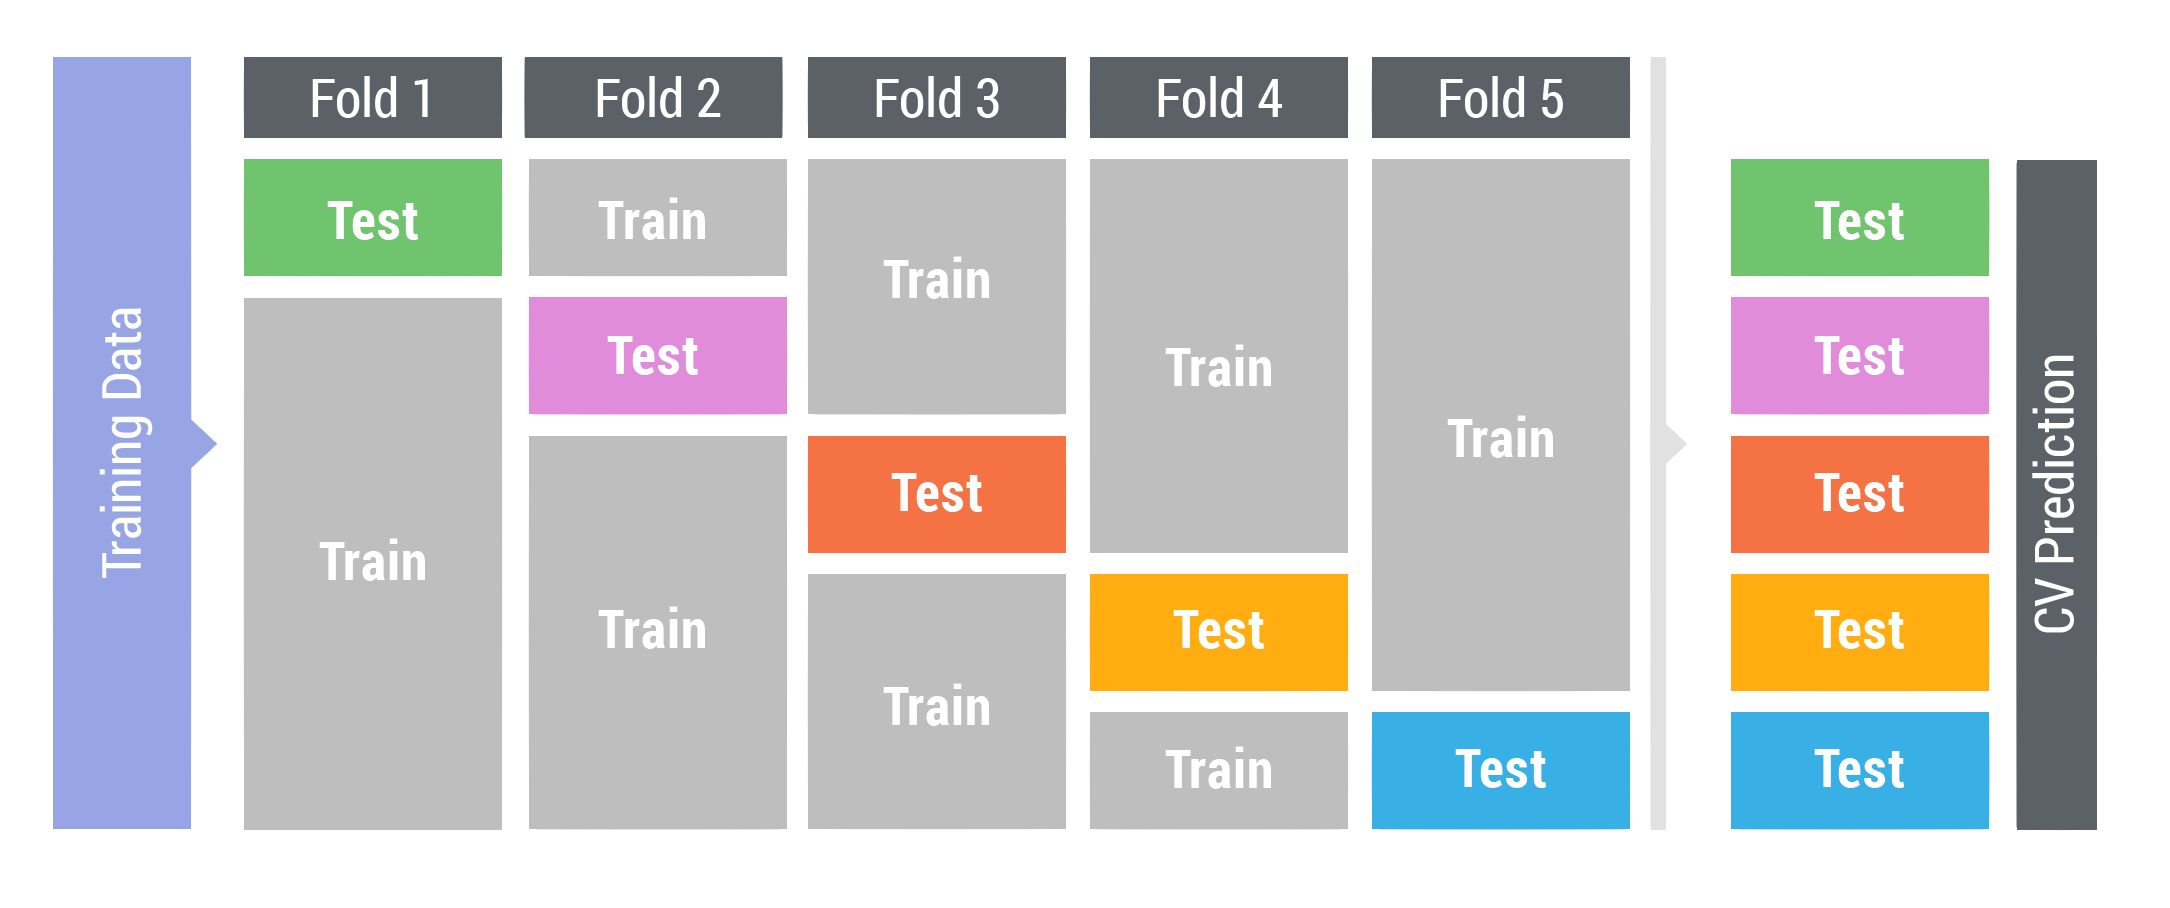
\includegraphics[width=0.5 \textwidth]{cv}
    \caption{5-fold CV.}
\end{figure}

We used stratified 5-fold cross validation (CV) for model validation and ensemble.
As shown in Figure 3, training data were split into 5 folds while the sample size and dropout rate were preserved across the folds.

For validation, each of single and ensemble models was trained 5 times. Each time, 1 fold was held out and the remaining 5 folds were used for training. Then, predictions for the hold-out folds were combined and formed the model's CV prediction. CV predictions were used as inputs for ensemble model training as well as the model's CV score calculation.

For test, each of single and ensemble models was retrained with whole training data. Then predictions for test data were used as inputs for ensemble prediction as well as for submission. 
